\documentclass[../main.tex]{subfiles}
\DeclareSIUnit\angstrom{\text{\r A}}

\graphicspath{{../images/}}

\begin{document}
\pagestyle{fancy}
\lhead{Lecture 15: 3/26}
\chead{Chapter 8}
\rhead{PHYS 472}

\section*{Chapter 14: Plasmons, Polaritons, and Polarons}
\addcontentsline{toc}{section}{Chapter 14: Plasmons, Polaritons, and Polarons}

\subsection*{E\&M Stuff} 
In E\&M, we extensively study two fields: the electric field $\vb E$ and the magnetic field $\vb B$.
We also have a vector
\begin{align*}
    \vb D = \vb E + 4\pi \vb P
\end{align*} 
where $\vb P$ is the polarization vector, and $\vb D$ is the displacement vector. In a static field,
we see that the divergence of the electric field
\begin{align*}
    \div \vb E = \frac{\rho}{\epsilon_0}
\end{align*}
is equivalent to the ratio of the charge density $\rho$ and the permittivity of free space
$\epsilon_0$. We also know that the curl
\begin{align*}
    \curl \vb E = 0
\end{align*}
is zero as the electric field can be expressed as the gradient of a scalar(Hemholtz) potential. 
Looking at the displacement vector,
\begin{align*}
    \div \vb D = 4\pi \rho_f
\end{align*}
where in CGS units we define
\begin{align*}
    \vb D = \epsilon \vb E
\end{align*}
where the dielectric function $\epsilon(\omega, \vb K)$ has a dependence on frequency and wave
vector which makes it a difficult problem to solve. 
\paragraph*{Plasmon} 
The total charge density
\begin{align*}
    \rho = \rho_{\text{ext}} + \rho_{\text{ind}}
\end{align*}
is the sum of the external charge density and the induced charge density. In CGS units, the 
divergence of the two fields are
\begin{align*}
    \div \vb D &= \rho_{\text{ext}} \\
    \div \vb E &= 4\pi(\rho_{\text{ext}} + \rho_{\text{ind}})\\
        &= 4\pi \rho
\end{align*}
We define the following
\begin{align*}
    D(\vb K) &= \epsilon(\vb K) \vb E(\vb K)
\end{align*}
so the divergence of the electric field and displacement vector are
\begin{align*}
    \div \vb E &= \div [\sum \vb E(\vb K) e^{i\vb K \cdot \vb r}] 
    = 4\pi \sum_K \rho(\vb K) e^{i\vb K \cdot \vb r} 
\end{align*}
and
\begin{align*}
    \div \vb D &= \div[\sum_K \epsilon(\vb K) \vb E(\vb K) e^{i\vb K \cdot \vb r}]
    = 4\pi \sum_K \rho_{\text{ext}}(\vb K) e^{i\vb K \cdot \vb r}
\end{align*}
diving the two equations we find
\begin{align*}
    \epsilon(\vb K) &= \frac{\rho_{\text{ext}}(\vb K)}{\rho(\vb K)}
     = 1 - \frac{\rho_{\text{ind}}}{\rho(\vb K)}
\end{align*}
\paragraph*{Free Electron} In 1D, the EOM of an electron in an electric field is
\begin{align*}
    m \dv[2]{x}{t} = - eE
\end{align*}
where time dependence is harmonic i.e.
\begin{align*}
    x &= x_0 e^{-i\omega t} \\
    \implies -\omega^2 m x_0 &= -eE;\qquad x_0 = \frac{eE}{m\omega^2}
\end{align*}
The polarization, or dipole moment per unit volume of the electron, is
\begin{align*}
    P = -nex_0 = \frac{ne^2E}{m\omega^2}
\end{align*}
where $n$ is the electron density. So the dielectric function is
\begin{align*}
    \epsilon(\omega) = \frac{D}{E} = \frac{E + 4\pi P}{E} = 1 - \frac{4\pi ne^2}{m\omega^2}
\end{align*}
We define the plasma frequency as
\begin{align*}
    \omega_p^2 = \frac{4\pi ne^2}{m} 
\end{align*}
so
\begin{align*}
    \epsilon(\omega) = 1 - \frac{\omega_p^2}{\omega^2}
\end{align*}
\paragraph*{Example} In the background the dielectric constant $\epsilon(\infty)$ then
\begin{align*}
    \epsilon(\omega) &= \epsilon(\infty)\qt[1 - \frac{\bar{\omega}_p^2}{\omega^2}]
\end{align*}
where
\begin{align*}
    \bar{\omega}_p^2 = \frac{4\pi ne^2}{m\epsilon(\infty)}
\end{align*}
\subsection*{Electromagnetic wave} 
From the Poynting vector
\begin{align*}
    \vb S = \vb E \cross \vb B
\end{align*} 
\paragraph*{Aside: 3 Types of Differential Equations}
\begin{itemize}
    \item The wave equation 
    \begin{align*}
        A\laplacian f = \pdv[2]{f}{t}
    \end{align*}
    \item The diffusion equation
    \begin{align*}
        D \laplacian f = \pdv{f}{t}
    \end{align*}
    \item The Poisson equation
    \begin{align*}
        \laplacian f = A
    \end{align*}
\end{itemize}
For EM waves, the wave equation is
\begin{align*}
    \dv[2]{D}{t} = c^2 \laplacian \vb E
\end{align*}
where we have a solution
\begin{align*}
    E \propto e^{i\omega t} e^{i\vb K \cdot \vb r}\qand \vb D = \epsilon \vb E
\end{align*}
so the wave equation tells us the dispersion relation
\begin{align*}
    \omega^2 \epsilon(\omega, \vb K) = c^2 K^2
\end{align*}
This tells us some intersting things
\begin{itemize}
    \item $\epsilon$ is real, $\epsilon > 0$, and for real $K$ and $\omega$ the wave propogates 
    transversely with phase velocity 
    \begin{align*}
        v_p = \frac{c}{\sqrt{\epsilon}}
    \end{align*}
    \item If $\epsilon$ is real and $\epsilon < 0$, then $K$ is imaginary and the wave is damped.
    \item If $\epsilon$ is complex and $\omega$ is real, $\vb K$ is complex and is damped.
\end{itemize}
From the dispersion relation
\begin{align*}
    \epsilon(\omega, \vb K) = 1 - \frac{\omega_p^2}{\omega^2}
\end{align*}
if $\omega < \omega_p$ there is total reflection, and if $\omega > \omega_p$ the material is 
transparent. 
\paragraph*{Metal} In a metal with positve charge density, we apply an electric field to slighlty
displace the electrons and cause them to oscillate. The EOM is
\begin{align*}
    n m \dv[2]{x}{t} = -neE
\end{align*}
This displaces the surface charge density $\sigma = \pm neu$ or a capacitor. Using a gaussian pillbox at the 
two surfaces of the capacitor, we know that
\begin{align*}
    E \cdot S = \frac{\sigma \cdot s}{\epsilon_0} = \frac{\sigma}{\epsilon_0}
\end{align*}
and from Gauss's law
\begin{align*}
    E = 4\pi n u e
\end{align*}
so the wave equation is
\begin{align*}
    nm\dv[2]{u}{t} = -neE = -4\pi ne^2 u \\
    \implies \dv[2]{u}{t} + \omega_p^2 u = 0
\end{align*}
where the frequency is
\begin{align*}
    \omega_p = \sqrt{\frac{4\pi ne^2}{m}}
\end{align*}
We can approximately find that for $10^{23}$ electrons per cubic centimeter(Avogadro's number) we 
get a frequency of roughly $10^{16}$ Hz, and the energy is roughly
\begin{align*}
    \hbar \omega_p \approx \frac{10^{-34} \cdot 10^{16}}{10^{-19}} = \qty{1}{eV}
\end{align*}
Experimentally we find that the plasmon energy is roughly $\qty{10}{eV}$ since the frequency is
$10^{16}$ Hz. 

\newpage
\lhead{Lecture 16: 3/28}
When $\vb K$ goes to zero, we look at the optical modes for the dielectric function, when $\omega$
goes to zero i.e. $\epsilon(0, \vb K)$, we find that the applied field is screened by the electrons.
\begin{align*}
    \epsilon(K) &= \frac{\Delta \rho}{\rho} = 1 - \frac{\rho_{\text{ind}}}{\rho} \\
    &= \frac{\varphi_{\text{ext}}}{\varphi}
\end{align*}
where $\varphi$ is the potential. The electron response has a perturbed density
\begin{align*}
    \rho(x) = -n_0 e + \rho_{\text{ind}}(\vb K)\sin(\vb K \cdot \vb x)
\end{align*}
And we use the Poisson equation for the total charge density
\begin{align*}
    \laplacian \varphi = -4\pi \rho
\end{align*}
but this depends on $\vb r$ so to solve this in terms of $\vb K$ we use the Fourier transform
\begin{align*}
    \int \psi(\vb K) e^{i\vb K \cdot \vb x} \dd{\vb K} \\
    \implies K^2 \psi(\vb K) = 4\pi \rho(\vb K)
\end{align*}
\paragraph*{Chemical Potential}
From the 3D fermi energy
\begin{align*}
    \epsilon_F = \frac{\hbar^2 k_F^2}{2m}
\end{align*}
we can find the chemical potential
\begin{align*}
    \mu = \epsilon_F^0 = \frac{\hbar^2}{2m} (3\pi^2 n_0)^{2/3}
\end{align*}
is perturbed by the potential $-e\varphi(x) \to n$ so
\begin{align*}
    \mu &= \epsilon_F^0 - e\varphi(x) = \frac{\hbar^2}{2m} (3\pi^2 n)^{2/3} - e\varphi(x)
\end{align*}
and we can solve for $e\varphi(x)$ and use Taylor expansion to find
\begin{align*}
    e\varphi(x) = \dv{\epsilon_F}{n_0} [n(x) - n_0] \quad \dv{\epsilon_F}{n_0} = \frac{2\epsilon_F}{3n_0} \\
    \implies n(x) - n_0 = \frac{3}{2} n_0 \frac{e\varphi(x)}{\epsilon_F}
\end{align*}
which is equivalent to the induced charge density
\begin{align*}
    \rho_{\text{ind}} = -\frac{3}{2} n_0 \frac{e^2}{\epsilon_F} \varphi(x) \\
    \implies \rho_{\text{ind}}(\vb K) = -\frac{3}{2} n_0 \frac{e^2}{\epsilon_F} \varphi(\vb K)
\end{align*}
and using
\begin{align*}
    k^2 \rho(\vb K) = 4\pi \rho(\vb K)
\end{align*}
we get
\begin{align*}
    \rho_{\text{ind}}(\vb K) = -\frac{6\pi n_0 e^2}{\epsilon_F K^2} \rho(\vb K)
\end{align*}
and the dielectric function is
\begin{align*}
    \epsilon(\vb K) = 1 - \frac{\rho_{\text{ind}}}{\rho} = 1 + \frac{6\pi n_0 e^2}{\epsilon_F K^2}
\end{align*}
Defining
\begin{align*}
    k_s^2 &= \frac{6\pi n_0 e^2}{\epsilon_F} \\
        &= 4 \qt(\frac{3}{\pi})^{1/3} \frac{n_0^{1/3}}{a_0}
\end{align*}
so
\begin{align*}
    \epsilon(\vb K) = 1 + \frac{k_s^2}{K^2}
\end{align*}
which is the Thomas-Fermi screening. This also means we have a screening length $1/k_s$.
\paragraph*{Screened Coulomb Potential} For a point charge the Poission equation is a delta function
\begin{align*}
    \laplacian \varphi = - 4\pi q \delta(\vb r) \implies \varphi_0 = \frac{q}{r}
\end{align*}
taking the Fourier transform of both sides
\begin{align*}
    \varphi_0(\vb r) = \frac{1}{(2\pi)^3} \int \dd{\vb K} \varphi_0 (\vb K) e^{i\vb K \cdot \vb r} \\
    \delta(\vb r) = \frac{1}{(2\pi)^3} \int \dd{\vb K} e^{i\vb K \cdot \vb r}
\end{align*}
So each fourier component is independent and we find
\begin{align*}
    \varphi(\vb K) = \frac{4\pi q}{K^2}
\end{align*}
since
\begin{align*}
    \epsilon(\vb K) = \frac{\varphi_{\text{ext}}}{\varphi} = 1 + \frac{k_s^2}{K^2} \\
    \implies \varphi(K) = \frac{4\pi q}{K^2} \frac{K^2}{K^2 + k_s^2} = \frac{4\pi q}{K^2 + k_s^2}
\end{align*}
And we find the screened potential by taking the Fourier transform
\begin{align*}
    \varphi(r) &= \frac{1}{(2\pi)^3} \int \dd{\vb K} \frac{4\pi q}{K^2 + k_s^2} e^{i\vb K \cdot \vb r} \\
    &= \frac{q}{r} e^{-k_s r}
\end{align*}
from the residue theorem. We can see that we have two decaying terms where the exponential term 
decays much faster, or the short regime. So we have the two cases
\begin{align*}
    \epsilon(\omega, 0) = 1 - \frac{\omega_p^2}{\omega^2} \quad \epsilon(0, K) = 1 + \frac{k_s^2}{K^2}
\end{align*}
\paragraph*{Metal-Insulator Transition} We'd expect that doping a metal with more impurities would
decrease the resistivity gradually. However, we find that the resistivity drops suddenly at a
critical concentration. As $k_s$ increases we move the bound state up in energy, and at a critical
point, the bound states overlap with the other wells and the system becomes a metal. A bare Coulomb
potential always has a bound state. For a delta function potential, there is only one bound state.

\newpage
\lhead{Lecture 17: 4/2}
\subsection*{Phonon in metal}
The T-F(Thomas-Fermi) screening of the dielectric function
\begin{align*}
    \epsilon(\vb K) = 1 + \frac{k_s^2}{K^2}
\end{align*}
approximates for an electron where at small $\lambda$ the the constant is $1$ or a vacuum. The 
plasma contribution from the ions gives us
\begin{align*}
    \epsilon(\vb K, \omega) = 1 + \frac{k_s^2}{K^2} - \frac{4\pi n e^2}{M\omega^2} \quad \omega_p^2 = \frac{4\pi n e^2}{M}
\end{align*}
For the long wavelength limit, we look at a short range in $K$ or
\begin{align*}
    k, \omega \ll 1
\end{align*}
so we can neglect the 1 term in the dielectric function, and looking at the dielectric function at
zero tells us the phonnon information (the excitation state of the lattice):
\begin{align*}
    \omega^2 = \frac{4\pi n e^2}{M k_s^2} K^2
\end{align*}
Replacing $k_s$ with the fermi energy $\epsilon_F$ we get 
\begin{align*}
    \omega^2 = \frac{4\pi n e^2}{M} \frac{\epsilon_F}{6\pi n e^2} K^2
\end{align*}
and using the fermi velocity $\epsilon_F = \frac{1}{2} m V_F^2$ 
\begin{align*}
    &= \frac{m}{3M} V_F^2 K^2 \\
    \omega &= \qt(\frac{m}{3M})^{1/2} V_F K \\
    \implies V &= \frac{\omega}{K} = \qt(\frac{m}{3M})^{1/2} V_F 
\end{align*}
where we $v$ is the sound velocity of the phonon in the metal. This describes how long wavelength 
phonons propogate in the metal. We can think of the plasmon and phonon to be a coupled system which
can be represented as a matrix equation
\begin{align*}
    \mqty(E_1 & \triangle \\ \triangle & E_2) \mqty(\text{plasmon} \\ \text{phonon}) = 0
\end{align*}
which has two solutions
\begin{align*}
    \mqty(\text{plasmon} \\ 0 ) \quad \mqty(0 \\ \text{phonon})
\end{align*}
And the plasmon has optical modes and the phonon has acoustic modes (longitudinal) which is
similar to the two dispersion relations as shown in the figure below.
\begin{figure}[ht]
    \centering
    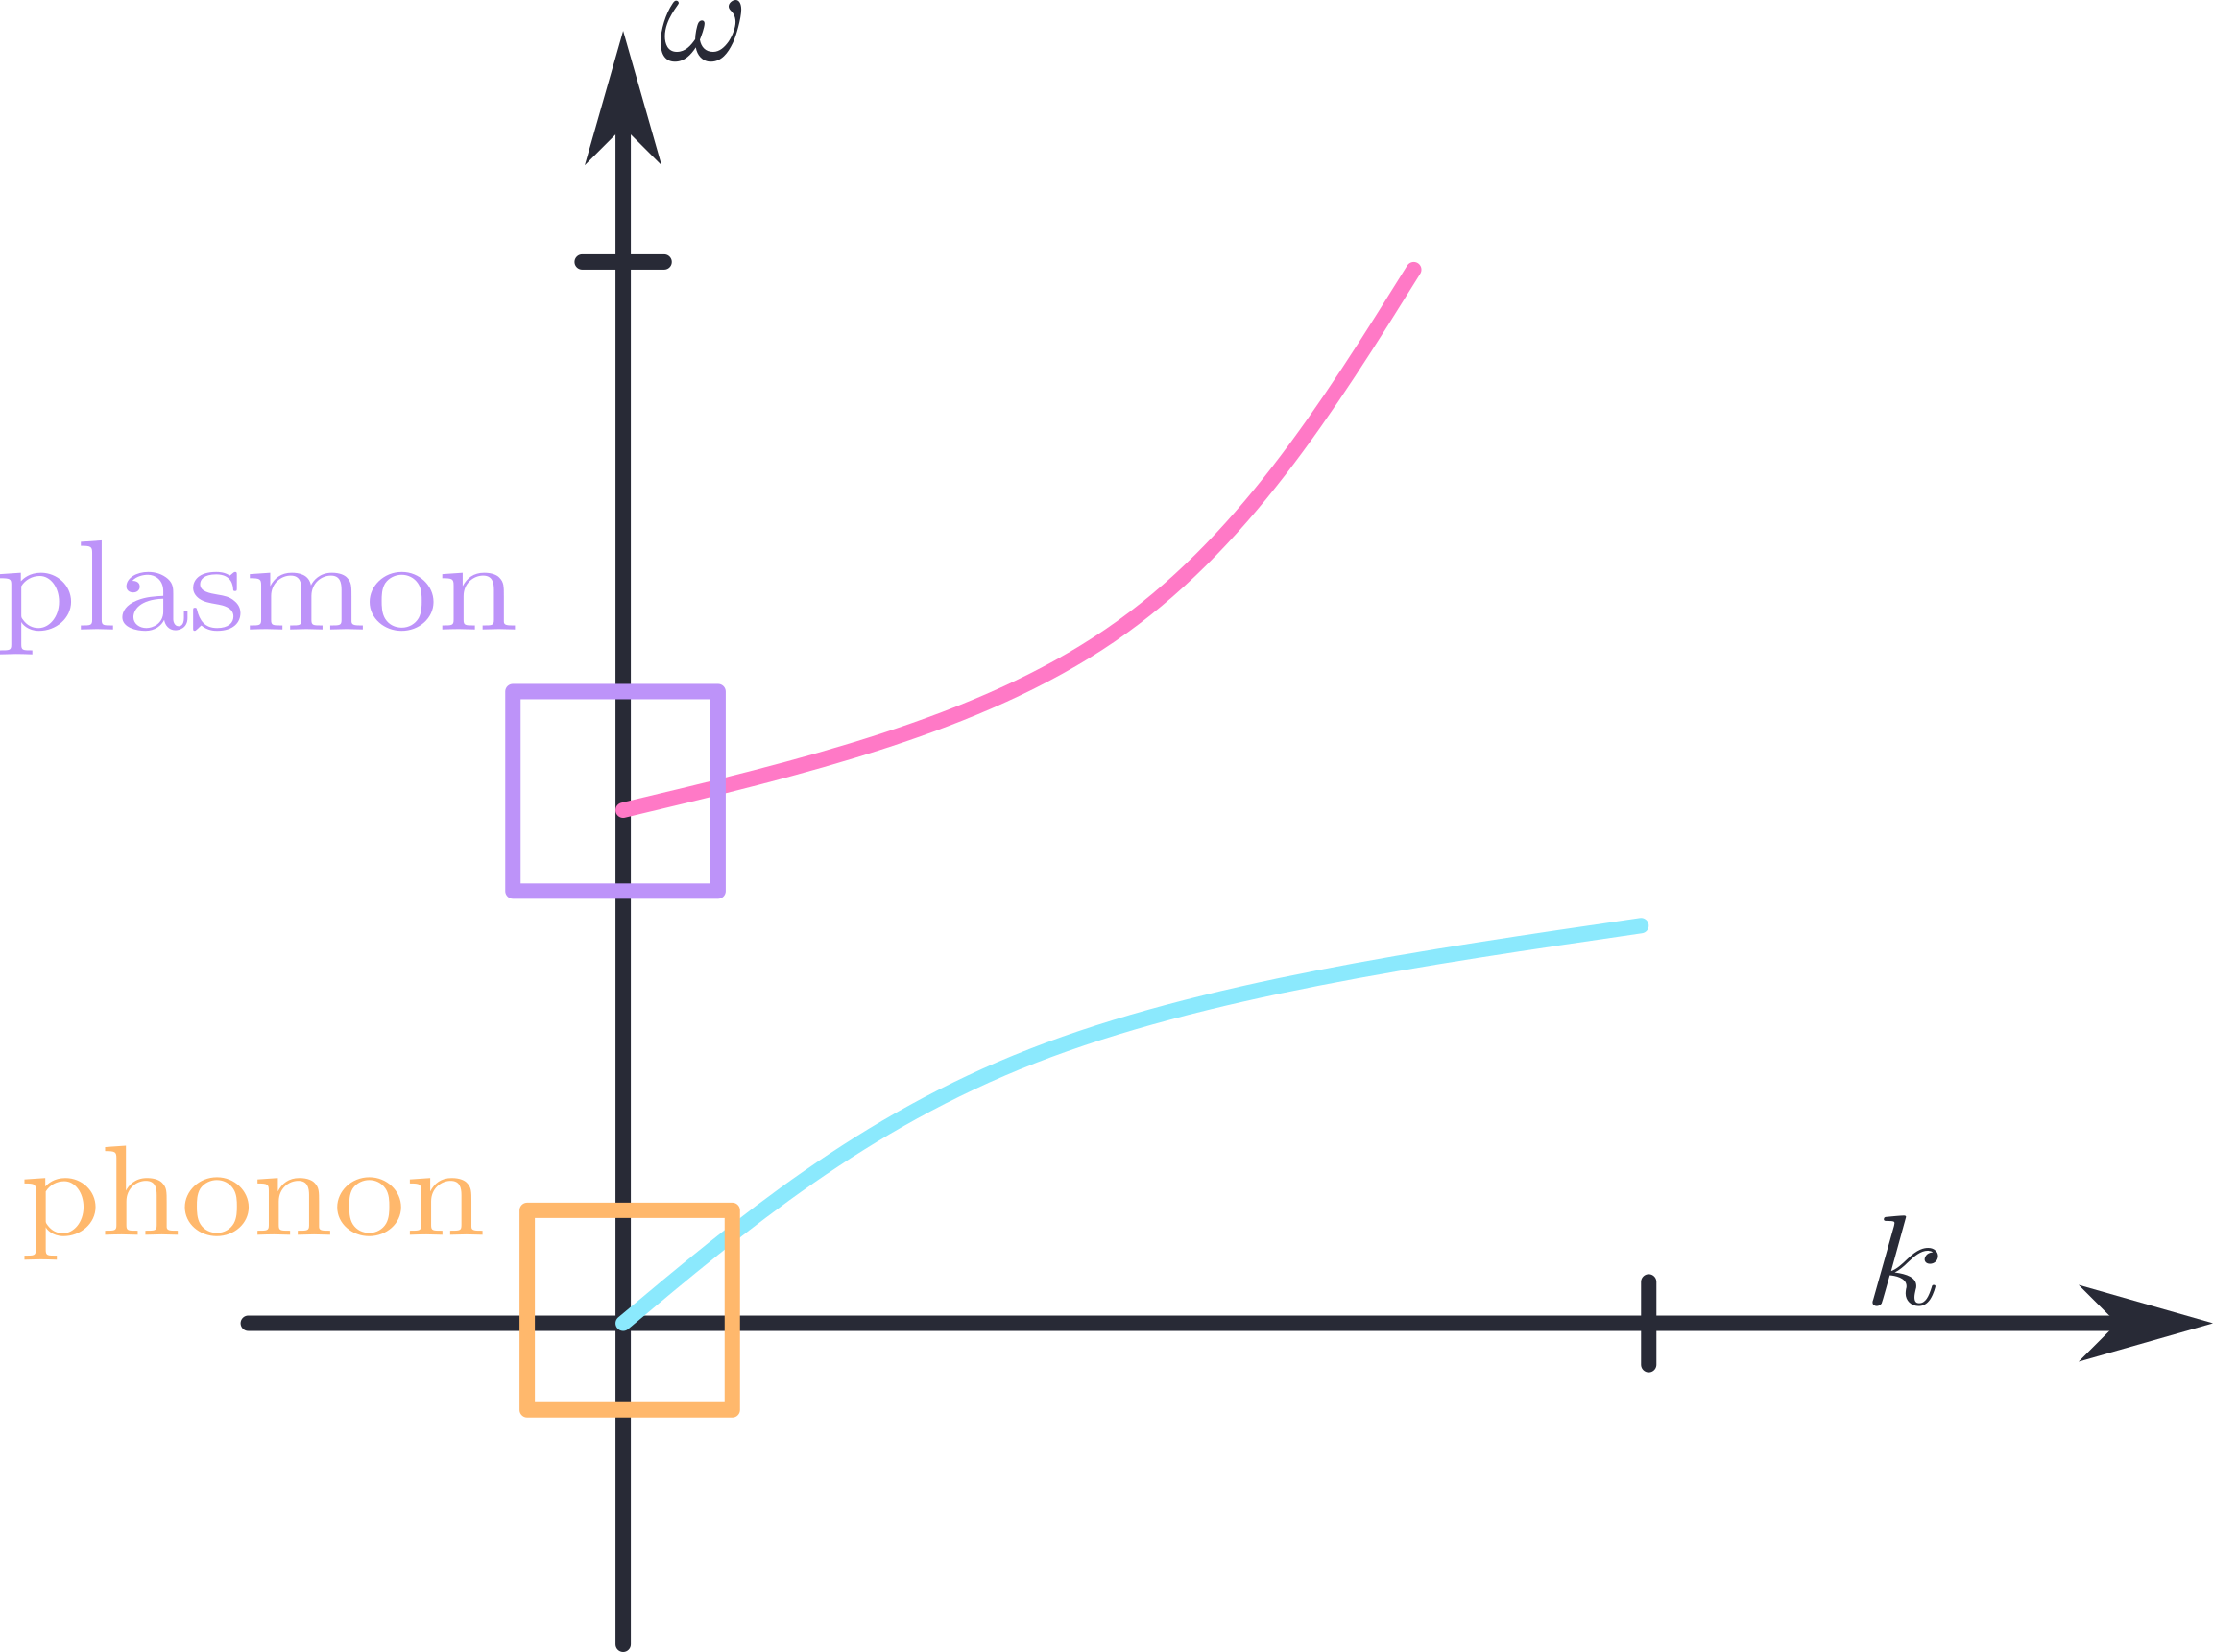
\includegraphics[width=0.5\textwidth]{plasmon_phonon.png}
    \caption{Phonon and Plasmon Dispersion Relations}
    \label{fig:phononplasmon}
\end{figure}

\subsection*{Polaritons}
From the wave equation
\begin{align*}
    \dv[2]{D}{t} = c^2 \laplacian \vb E
\end{align*}
and we know that the wavelike nature of E\&M waves so
\begin{align*}
    E,D \sim e^{i\omega t} e^{i\vb E \cdot \vb r} \\
    D = E + 4\pi P \\
    D = \epsilon E
\end{align*}
so
\begin{align*}
    \omega^2 [E + 4\pi P] = c^2 k^2 E
\end{align*}
And from Newtons laws, we know that the displacement of the positive ions are given by
\begin{align*}
    M \dv[2]{u}{t} = -\pdv{V}{u}
\end{align*}
With two equations and two unknowns, we have a matrix equation where
\begin{align*}
    \mqty(E \\ P) \implies \begin{vmatrix}
        \omega^2 - c^2 k^2 & 4\pi \omega^2 \\
        \frac{Nq^2}{M} & \omega^2 - \omega_T^2
    \end{vmatrix}
    = 0
\end{align*}
which gives the equation
\begin{align*}
    -\omega^2 P + \omega_T^2 P = \frac{Nq^2}{M} E
\end{align*}
And the two solutions are at $\omega \to 0, k \to 0$ thus
\begin{align*}
    \omega = 0, \quad \omega^2 = \omega_T^2 + \frac{4\pi N q^2}{M}
\end{align*}
For light in EM we have the relation $\omega = ck$ which is a photon like branch in the dispersion
relation in Figure \ref{fig:phononplasmon}. So the polariton relates to the separate top branch. 

\paragraph*{Lydane-Sachs-Teller Relation} (LST)
\begin{align*}
    \frac{\omega_L^2}{\omega_T^2} = \frac{\epsilon(\omega = 0)}{\epsilon(\infty)}
\end{align*}
where $\epsilon(0)$ has the ion and electron part, and $\epsilon(\infty)$ or at very high frequency
the electron part dominates as the heavy ions are not able to respond to the high frequency. For 
4 atoms in a 3D unit cell so we have $3N = 12$ phonon modes, so 9 optical modes and 3 acoustic modes.
LO (longitudinal optical) lie below the TO (transverse optical) phonons 

\paragraph*{Electron + phonon = Polaron} In a crystal lattice, we have a mobility of the electron
\begin{align*}
    j = \frac{ne^2 \tau}{m} E
\end{align*}
(Read about adiabatic approximation) In materials, the mobility is much less than the free electron.
The lattice structure distorts the motion of the electron which gives rise to the polaron. 
Photocatalytic water splitting tries to use light to split water into hydrogen. 

\newpage
\lhead{Lecture 18: 4/4}
\paragraph*{Optical Absorption} A photon of energy $\hbar \omega$ and momentum $\hbar k$ ($\omega = ck$)
absorbed in the electron band will excite an electron to move up into the conduction band. 
For a 1eV band gap, the wavelength is roughly
\begin{align*}
    \lambda = \frac{hc}{E} \approx \qty{1000}{nm}
\end{align*}
so the wave vector is $k = \frac{2\pi}{\lambda}$ in comparison to the lattice spacing
$\frac{2\pi}{a}$ where $a \approx \qty{0.1}{nm}$ we can see that the lattice spacing is much
larger than the wave vector. 
\begin{figure}[ht]
    \centering
    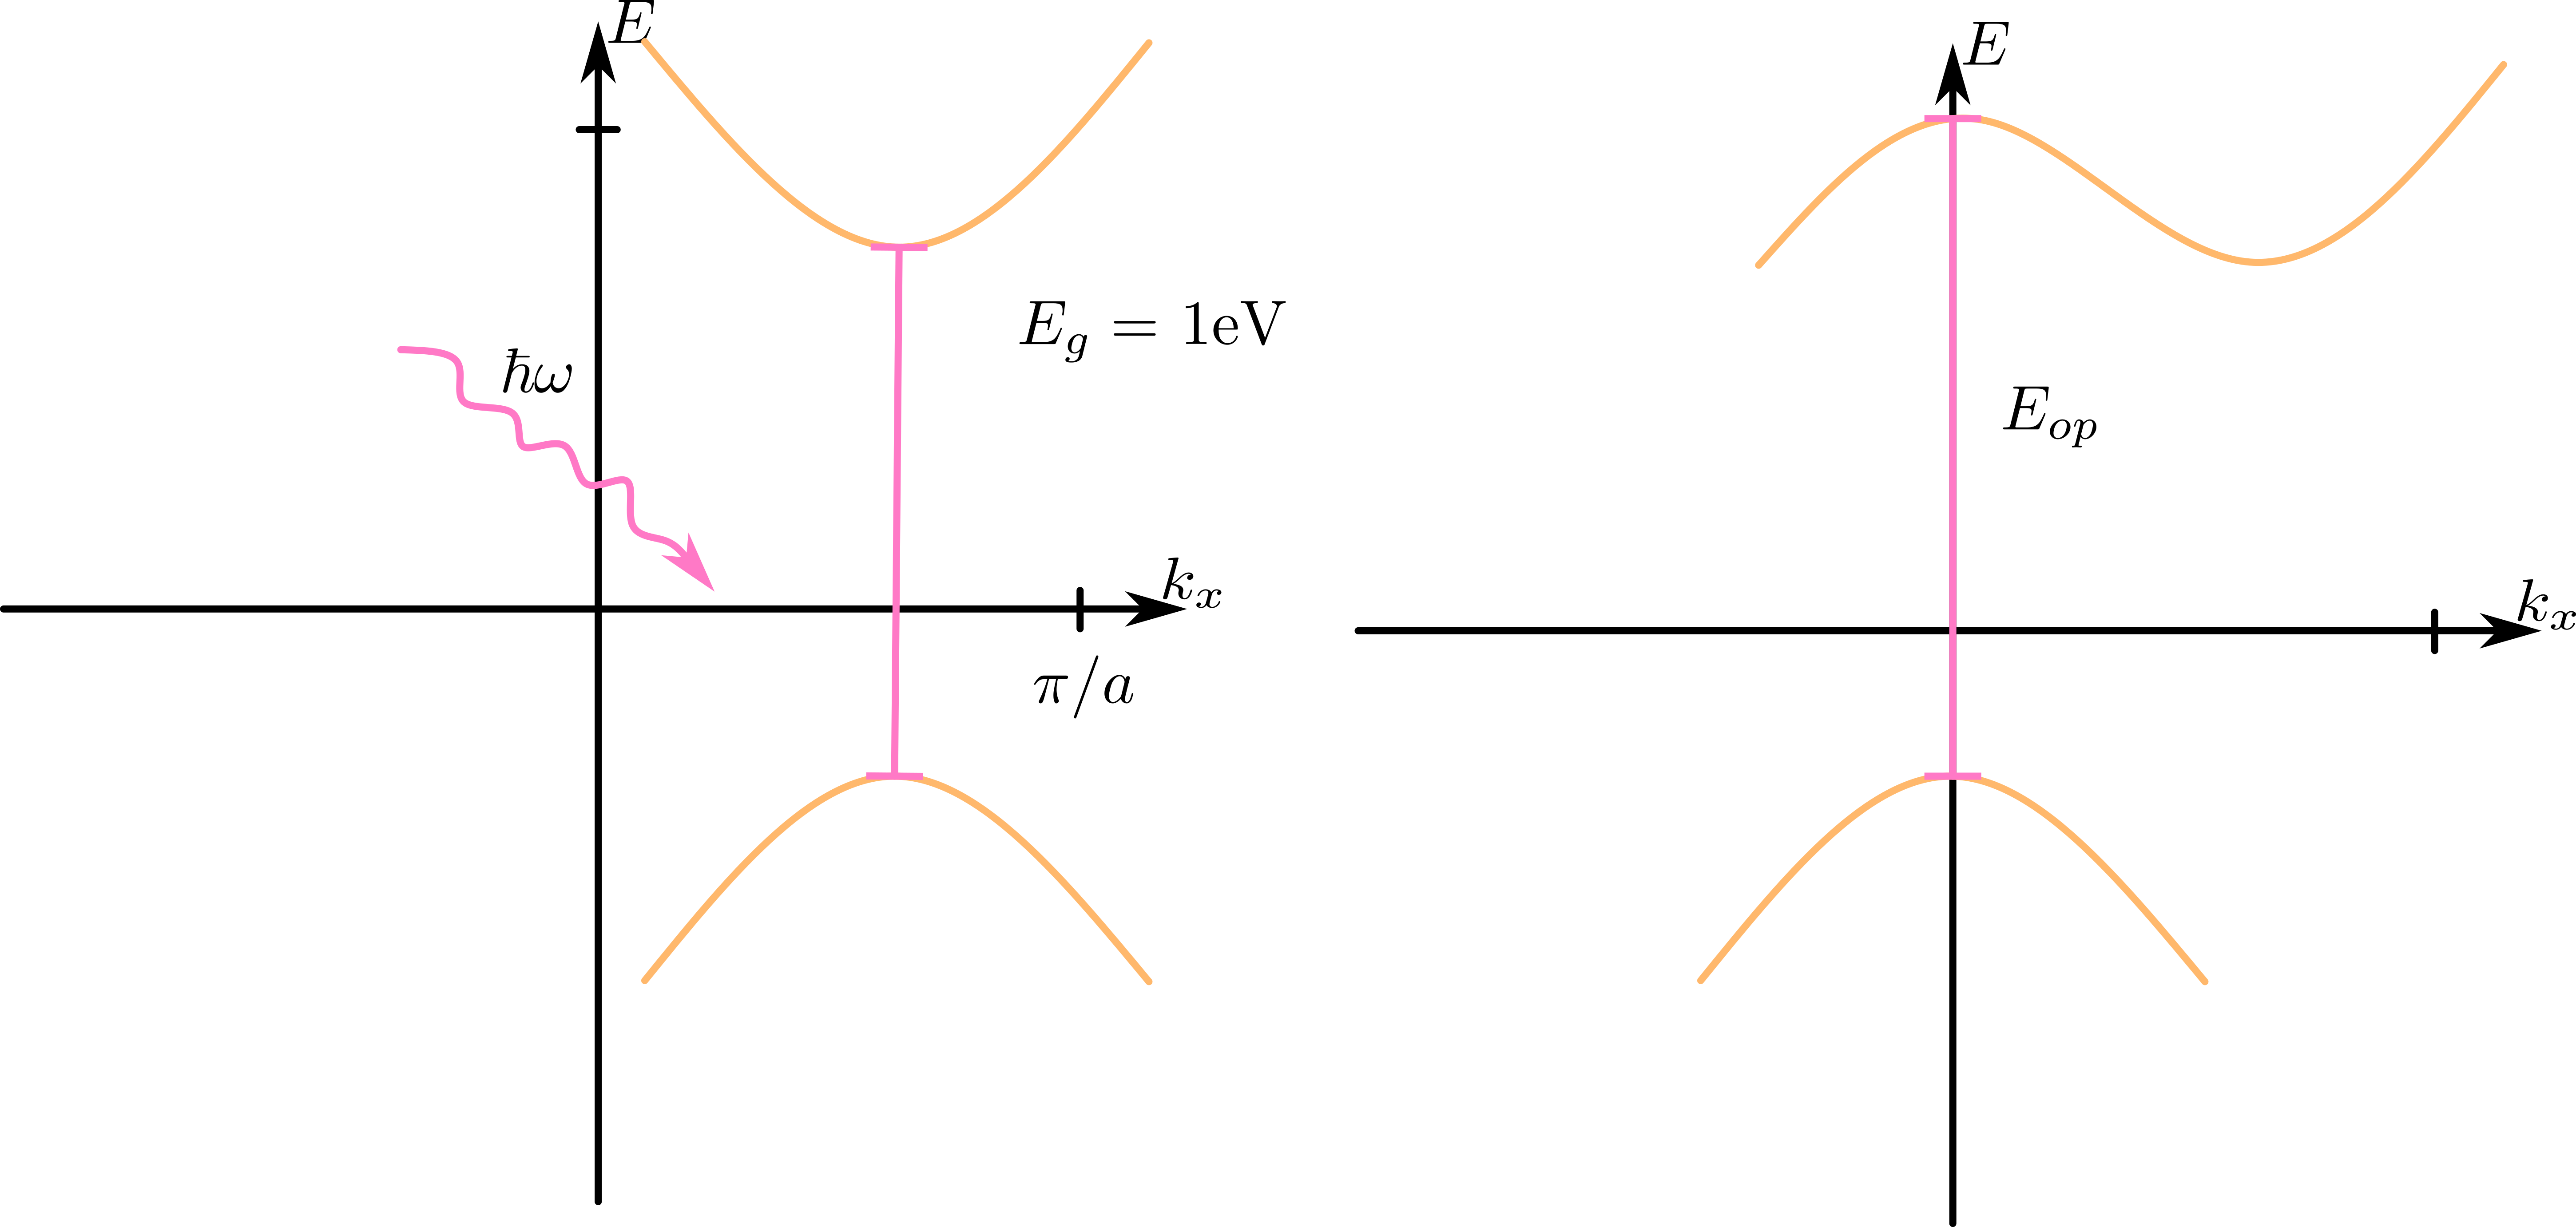
\includegraphics[width=0.8\textwidth]{bandgap.png}
    \caption{The left shows a direct band gap. The right shows indirect band gap.}
    \label{fig:bandgap}
\end{figure}
\paragraph*{LED} A current will inject holes in the bottom band and electrons in the top band, and 
the recombination of the two will emit a photon. For the indirect band gap, the holes build up near
the top of the valence band, and the phonon carries the momentum as the system recombines. The 
phonon will vibrate and heat up the system. The phonon of roughly $\qty{10}{meV}$ is small in 
comparison to the photon. 
\begin{itemize}
    \item photon takes energy
    \item phonon takes momentum
\end{itemize}
\paragraph*{Dirac Notation} The valence state $\ket{v}$ and the conduction state $\ket{c}$ we can 
represent the displacement of the two states with
\begin{align*}
    \bra{v}{\vb r \text{ dipole}} \ket{c}
\end{align*}
The absorption spectrum has several peaks, but we can approximate the absorption spectrum with a
smoothed Gaussian distribution. Each transition relates to the individual peaks, so we can take the
sum or
\begin{align*}
    \sum \abs{\bra{v}{\vb r \text{ dipole}} \ket{c}}^2
\end{align*}
The absorption will be proportional to the density of states and the strength of the dipole 
oscillator strength. If the valence and and conduction states have the same parity, the product
(whether even or odd) will be even. So $\vb r$ is odd annd we get a zero. We usually look at the
valence band as a p orbital(odd) and the conduction band as an s orbital(even). 

\newpage
\paragraph*{Emission Spectrum at Low Temperature}
\begin{figure} [ht]
    \centering
    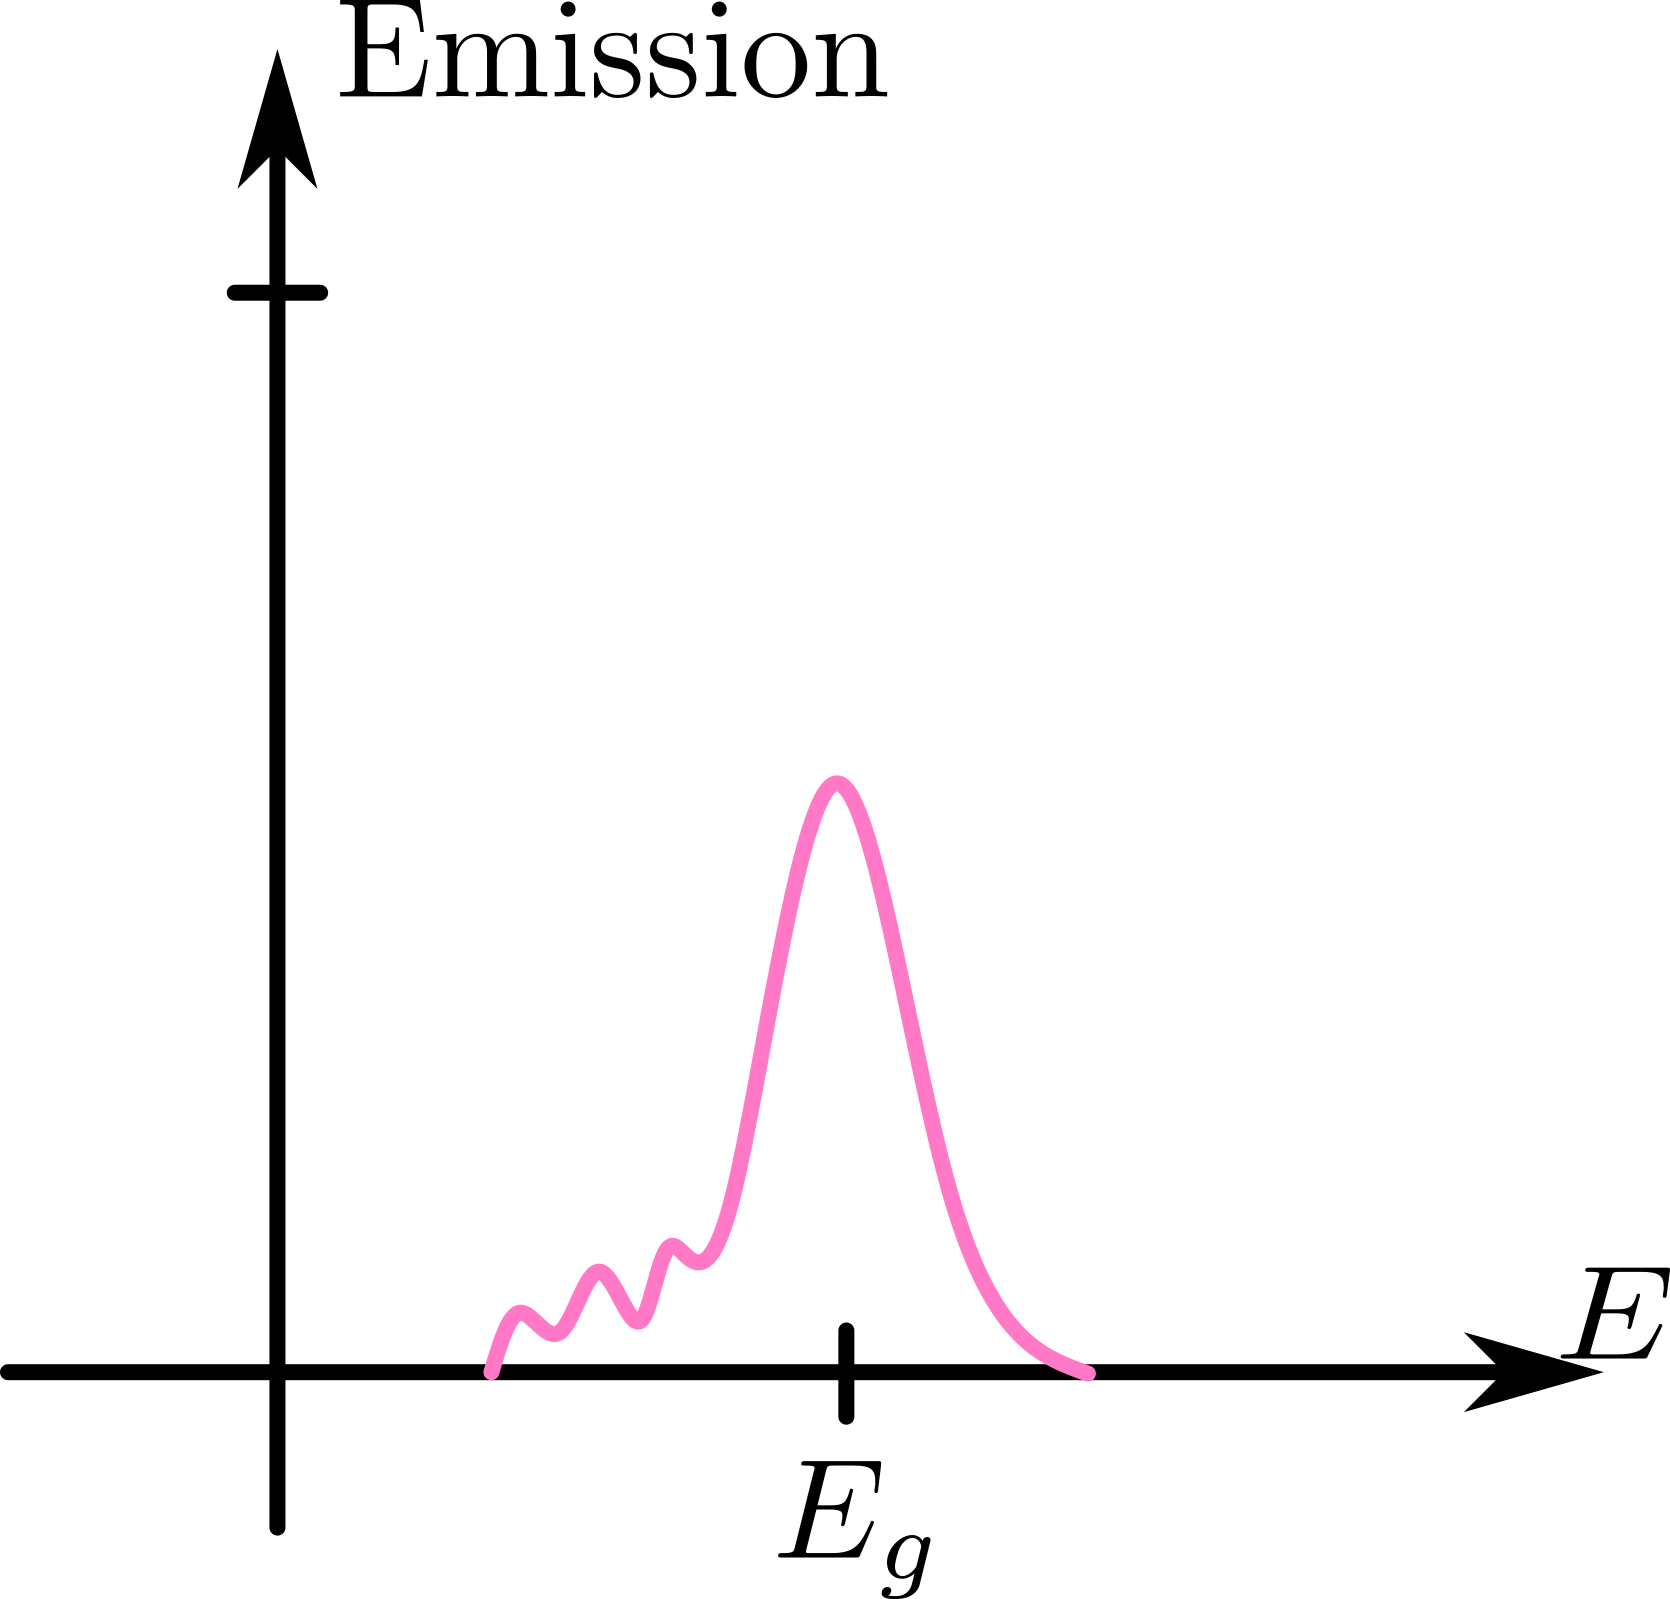
\includegraphics[width=0.5\textwidth]{emission.png}
    \caption{The emission spectrum at low temperature.}
    \label{fig:emission}
\end{figure}
We can see small peaks from the phonon excitation from experimental data (Stokes Shift). 
\begin{figure} [ht]
    \centering
    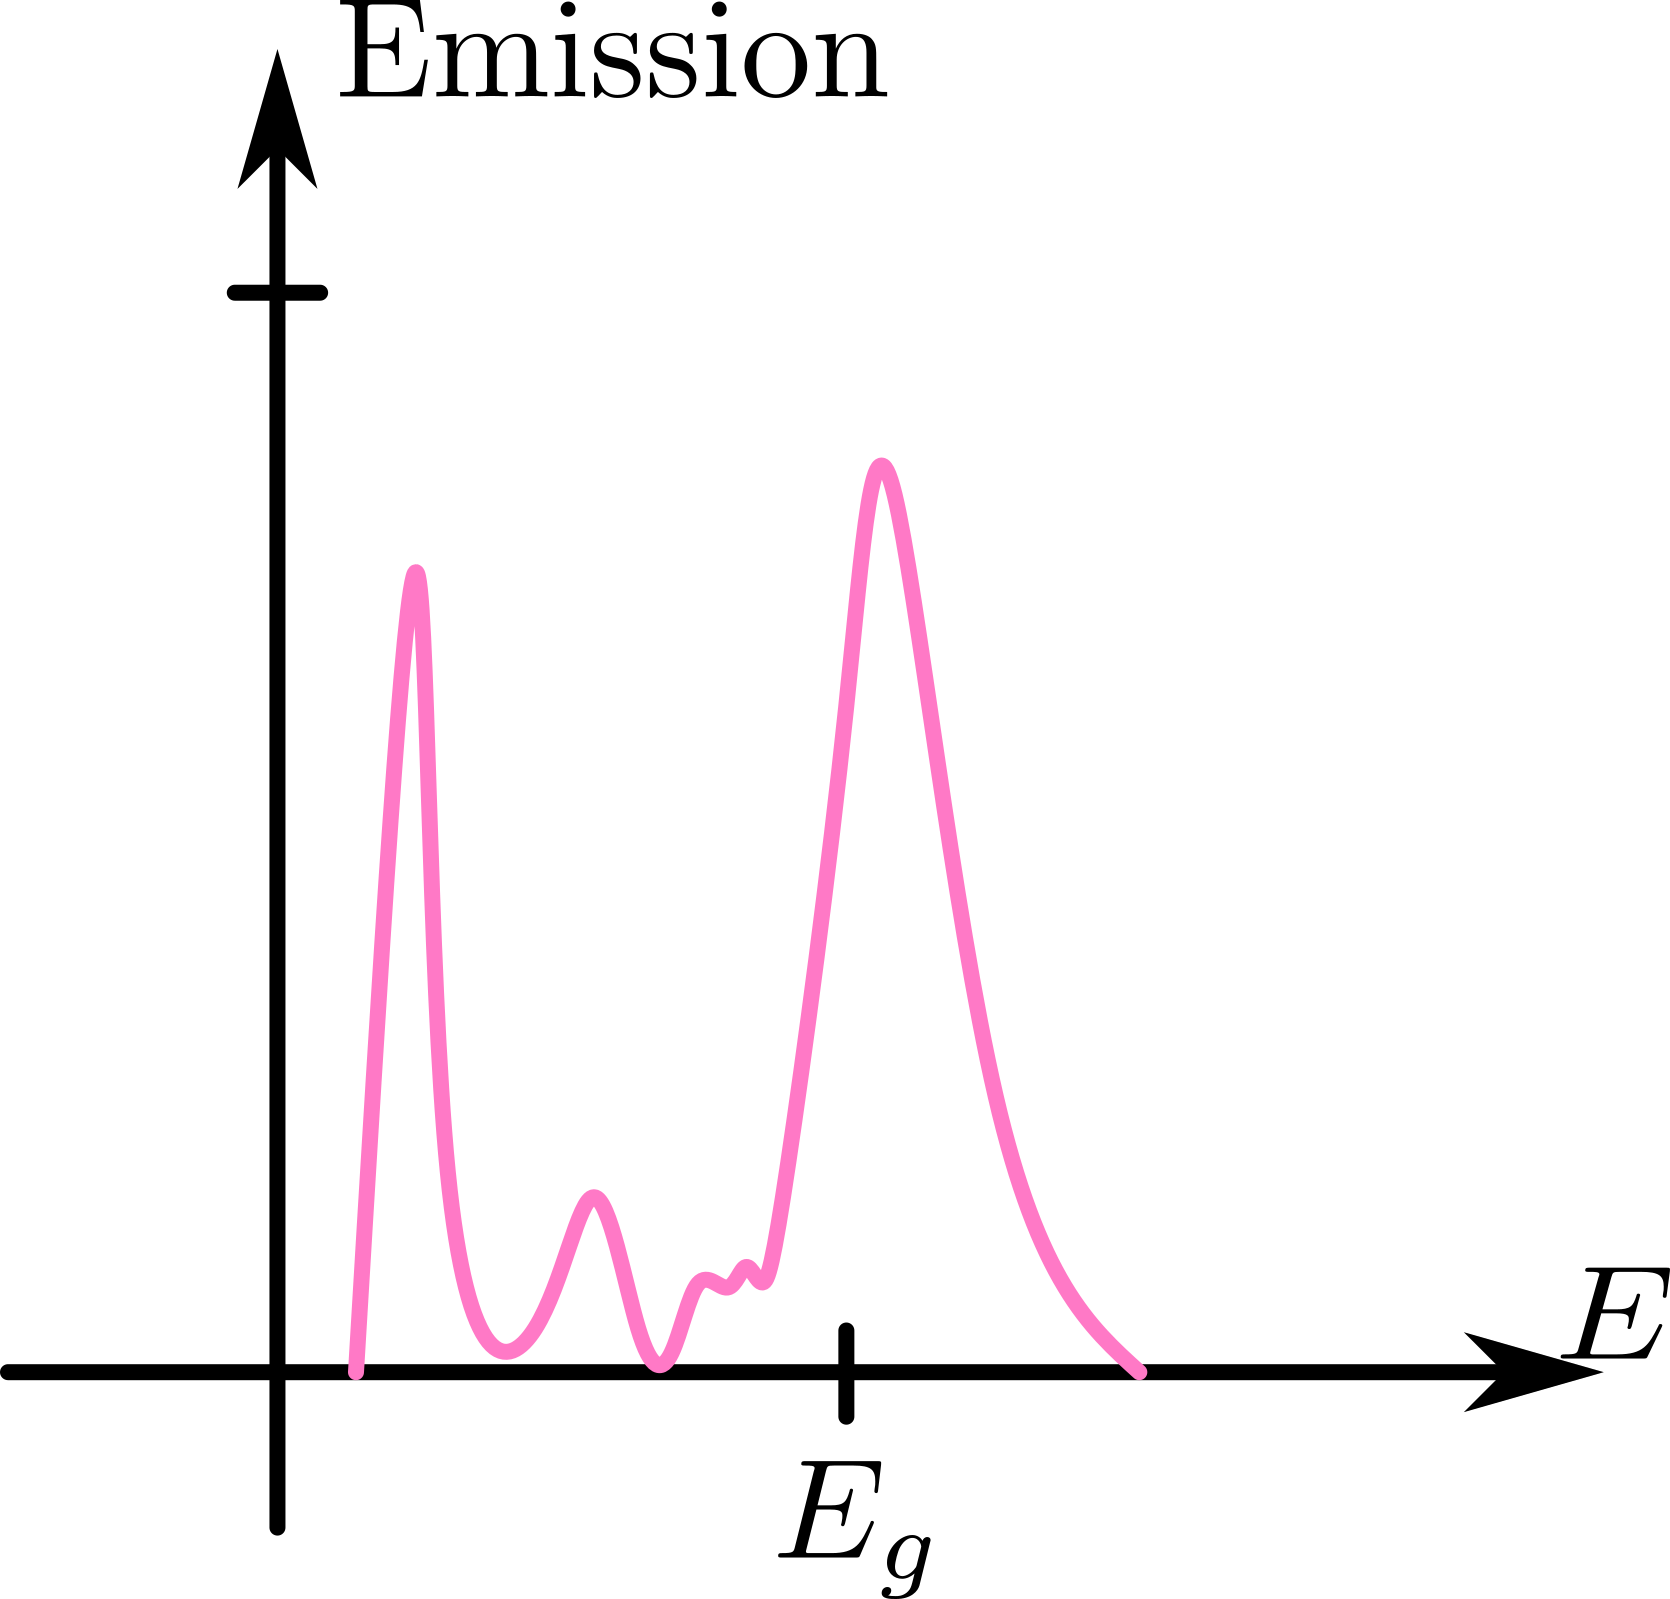
\includegraphics[width=0.5\textwidth]{emissionrevised.png}
    \caption{The emission spectrum at low temperature has a large peak at low energy.}
    \label{fig:emissionrevised}
\end{figure}
The electron hole pair have a bound state which has a binding energy of roughly $\qty{10}{meV}$ (
the gap between the first peak and the gap energy). 
\paragraph*{Hydrogen Model} The Rydberg energy for a hydrogen atom is
\begin{align*}
    \frac{m_0 e^4}{8 \epsilon_0^2 \hbar^2} = \qty{13.6}{eV} = \qty{1}{Ry}
\end{align*}
In a material the mass and dielectric constant change, i.e., the effective mass and dielectric
constant of a material. For silicon $\epsilon_0 \approx 10$ and the effective mass is
\begin{align*}
    m_e^* \approx 0.1 m_e
\end{align*}
or from the curvature of the energy band
\begin{align*}
    m \propto \frac{1}{\dv{^2 \epsilon}{k^2}}
\end{align*}
For silicon, we have a reduced mass for the electron hole pair
\begin{align*}
    \frac{1}{m_0} = \frac{1}{m_e} + \frac{1}{m_h}
\end{align*}
but the dispersion is anisotropic\dots the top down view of the valence band is oval shaped.
The approximation for the mass went from taking the average to a cyclotron mass:
\begin{align*}
    \frac{m_x + m_y}{2} \to m = \sqrt{m_x m_y}
\end{align*}
\paragraph*{Wavefunction}
For the wavefunction of the electron hole pair $\psi(x_e, x_h)$ we could have an s-orbital with a 
size of radius $\qty{100}{nm}$. This is kind of related to the binding energy 10 meV to the hydrogen
atom Rydberg energy of $\qty{13.6}{eV}$, so the binding energy is much smaller thus the larger size.

\paragraph*{Exciton} To get an exciton (electron hole pair) we need to have a lot of pairs that
contribute to the effective mass. 

\newpage
\section*{Quantum Mechanics in Materials} Fun Lecture

\paragraph*{}
Simulation + Novel Materials = New Quantum Properties, Materials and Applications

\begin{itemize}
    \item Novel Materials: Carbon Nanotube, Bucky Ball\dots
    \item Quantum Excitation: Nature is boring, and we can only observe things that are `excited'.
    \item High pressure: Metal-Insulator Transition
    \item Similar Electron and hole group velocity: Exciton (electron hole pair) 
    \item DFT (Density functional theory): Understimates band gap
    \item GW approximation improves on the theoretical to experimental band gap by asserting the 
    screening effect which reduces the coulomb interaction. 
    \item Exciton Insulators: Condensation of excitons
    \item Exciton have an attractive force which leads to a red shift (lowering) of the band gap.
    \item Qdots: Smaller sizes become more blue shifted because of the quantum confinement effect:
    \item Nanowires with Silicon.
    \item Experiment usually gets smaller exciton binding energy because of a substrate
\end{itemize}

\newpage
\section*{Chapter X: Magnetism}
\chead{Chapter X}
\lhead{Lecture 21: 4/16}
\paragraph*{Mermin Chapter 32 $\sim$ pg. 680}
For $T = 0$ We have many different types of magnetism:
\begin{itemize}
    \item Paramagnetism: Random unaligned spins, but the net magnetization is in one direction (PM)
    \item Ferromagnetism: All spins aligned in the same direction (FM)
    \item Antiferromagnetism: Neighboring spins are anti-aligned: N\'eel Vector (AFM)
\end{itemize}
\paragraph*{Real Materials}
Real materials prefer a magnetic moment in the plane of the material, but is there a ground state?
For a 2D material the magnetic moment lies in the $XY$ plane e.g. $CrCl_3$ or meron.
At finite temperatures, there are spin defects(spins that are not aligned) or vertex defects and
increase as the temperature increases. 

\paragraph*{Interaction between Spin}
Using the magnetic moment, we can calculate the interaction between to spins. The dipole-dipole
interaction
\begin{align*}
    U = \frac{1}{r^3} [\vb m_1 \cdot \vb m_2 - 3(\vb m_1 \cdot \vu r)(\vb m_2 \cdot \vu r)] \\
    \quad \vb m_1 = \frac{e\hbar}{mc} \quad  \vb r \approx \qty{1}{\angstrom}
\end{align*}
where this potential is roughly $\qty{0.1}{meV}$ and is much smaller than the room temperature
energy of $\qty{25}{meV}$. 

\paragraph*{1D Chain} We can not have a long range order in a 1D chain using the Ising model, so
we can not have a ferromagnetic state. At 1D the Curie Temperature is $T_c = 0$, so we do not 
have a stable state. 

\paragraph*{2D Ising Model} We can analytically solve the 2D Ising model as Onsager did using
transfer matrix methods.

\paragraph*{Hamiltonian}
\begin{align*}
    H = \sum{i,j} J \vb S_i \cdot \vb S_j 
\end{align*}
For when $J >0$ we have an AFM state, and when $J < 0$ we have a FM state. The energy difference
of the two states of spins are
\begin{align*}
    \bra{\uparrow \uparrow} H \ket{\uparrow \uparrow} - \bra{\uparrow \downarrow} H \ket{\uparrow \downarrow} = E_1 - E_2 \sim J
\end{align*}
From the wavefunction of the states
\begin{align*}
    \Psi = \psi(\vb r) \cdot \chi(\vb S)
\end{align*}
we know the fermion wf is antisymmetric (Pauli Exclusion Principle), so the wavefunction must
overlap in the local space, i.e. $J$ is short-range (exchange interaction). We call this because we
change the spin of the electron which results in a change in the energy states.

\paragraph*{Example:} A two electron system. The Hamiltonian is 
\begin{align*}
    H \psi &= - \frac{\hbar^2}{2m} [\laplacian_1 + \laplacian_2] \Psi + V(\vb r_1, \vb r_2) \Psi \\
    &= E \Psi
\end{align*}
where the total wavefunction is
\begin{align*}
    \Psi = \psi(\vb r) \phi_s
\end{align*}
The total spin is either 0 or 1, and the $z$ component of the spin is either $0$ or $\pm 1$:
\begin{center}
        \begin{tabular}{c|c|c}
            \hline
            $S$ & $S_z$ & $\chi$ \\
            \hline
            0 & 0 & $\frac{1}{\sqrt{2}} [\ket{\uparrow \downarrow} - \ket{\downarrow \uparrow}]$ \\
            \hline
            1 & 1 & $\ket{\uparrow \uparrow}$ \\
            1 & 0 & $\frac{1}{\sqrt{2}} [\ket{\uparrow \downarrow} + \ket{\downarrow \uparrow}]$ \\
            1 & -1 & $\ket{\downarrow \downarrow}$ \\
            \hline
        \end{tabular}
\end{center}
Where the singlet state is antisymmetric (minus sign) and the triplet state is symmetric. For the
model with two hydrogen atoms, neglecting the electron-electron interaction, we have
\begin{align*}
    (h_1 + h_2) \psi(\vb r_1, \vb r_2) = E \psi(\vb r_1, \vb r_2)
\end{align*}
where the Hamiltonian is
\begin{align*}
    h_i = -\frac{\hbar^2}{2m} \laplacian_i - \frac{e^2}{\abs{\vb r_i - \vb R_1}}
        - \frac{e^2}{\abs{\vb r_i - \vb R_2}}
\end{align*}
This implies the symmetric solution
\begin{align*}
    \psi_s (\vb r_1, \vb r_2) = \psi_0 (\vb r_1) \psi_0 (\vb r_2)
\end{align*}
where $\psi_0$ is an eigenstate of $h_i$. The antisymmetric solution
\begin{align*}
    \psi_t (\vb r_1, \vb r_2) = \frac{1}{\sqrt{2}} [\psi_0 (\vb r_1) \psi_1 (\vb r_2) - \psi_1 (\vb r_1) \psi_0 (\vb r_2)]
\end{align*}
Slater Determinant: 
\begin{align*}
    \mqty(\psi_1(r_1) & \psi_2 & \psi_3 \\ \psi_1(r_2) & \psi_2 & \psi_3) = 
\end{align*}
The symmetric state is the ground state because it has a lower energy. So the two states are
\begin{align*}
    \psi_0 &= \phi_1 (\vb r_1) + \phi_2 (\vb r_2) \\
    \psi_1 &= \phi_1 (\vb r_1) - \phi_2 (\vb r_2)
\end{align*}
The singlet state is
\begin{align*}
    \psi_s(\vb r_1, \vb r_2) = \phi_1 (\vb r_1) \phi_2 (\vb r_2) + \phi_2 (\vb r_1) \phi_1 (\vb r_2) \\
    + \phi_1 (\vb r_1) \phi_1 (\vb r_2) + \phi_2 (\vb r_1) \phi_2 (\vb r_2)
\end{align*}
where the last two terms are roughly zero (Heitler-London Approximation), and the Triplet state
\begin{align*}
    \psi_t(\vb r_1, \vb r_2) = 2 [ \phi_2 (\vb r_1) \phi_1 (\vb r_2) - \phi_1 (\vb r_1) \phi_2(\vb r_2)]
\end{align*}

\newpage
\lhead{Lecture 22: 4/18}
\paragraph*{H-L Approximation} 
So the energry difference of the singlet and triplet state is
\begin{align*}
    E_s - E_t &= \frac{\bra{\psi_s} \hat H \ket{\psi_s}}{\braket{\psi_s} }
     - \frac{\bra{\psi_t} \hat H \ket{\psi_t}}{\braket{\psi_t}} \\
    &\propto \int \dd{\vb r_1} \dd{\vb r_2} [\phi_1 (\vb r_1) \phi_2(\vb r_2)]
    [\phi_2(\vb r_1) \phi_1(\vb r_2)] \\
    &\qt[
        \frac{e^2}{\vb r_1 - \vb r_2} + \frac{e^2}{\abs{\vb R_1 - \vb R_2}} 
        - \frac{e^2}{\abs{\vb r_1 - \vb R_2}} - \frac{e^2}{\abs{\vb r_2 - \vb R_2}} 
    ]
\end{align*}
This is the exchange interaction, and not the Coulomb interaction, and is what reduces the
attractive forces between the electrons. 

\paragraph*{Heisenberg Model}
The Hamiltonian
\begin{align*}
    H^{\text{spin}} = \frac{1}{4} (E_s + 3E_t) - (E_s - E_t) \vb S_1 \cdot \vb S_2
\end{align*}
where the eiegenvalue of the triplet state is $E_t$:
\begin{align*}
    H^{\text{spin}} \ket{\uparrow \uparrow} = E_t \ket{\uparrow \uparrow}
\end{align*}
This also gives us the exchange interaction between the two spins
\begin{align*}
    H^{\text{spin}} = - (E_s - E_t) \vb S_1 \cdot \vb S_2 = - J \vb S_1 \cdot \vb S_2
\end{align*}
where $J$ is the exchange interaction. In a hexagonal latttice we have a Hamiltonian
\begin{align*}
    H = - \sum_{ij} J \vb S_i \cdot \vb S_j
\end{align*}
where we have 3 nearest neighbors and 6 next nearest neighbors for $J$. In all $\vu z$ we can
describe the ferromagnetic states (FM). 
\paragraph*{Example:} $\mathrm{CrI}_3$ (Hexagonal Structure) we find that the exchange interaction is
\begin{align*}
    J_1 = 2.12, \quad J_2 = 0.35, \quad J_3 = 0.05
\end{align*}
which decreases exponentially. For the other similar materials,
\begin{align*}
    \mathrm{CrBr}_3: J_1 &= 1.35, \quad J_2 = 0.14 \\
    \mathrm{CrCl}_3: J_1 &= 0.8, \quad J_2 = 0.07
\end{align*}
This decrease in $J$ comes from the spin-orbital coupling, or the mass of the element leads to a
stronger exchange interaction. Which one would have a higher Curie Temperature? The stronger 
interaction or $J$ would require a higher Curie Temperature $T_c$ to change from a FM to a PM state.

\paragraph*{Temperature Dependence} To get the temperature dependence, we use a monte carlo method
to simulate random spins assigned to a lattice. 
\begin{itemize}
    \item As the Temperature gets close to Curie temperature 
    but not quite there $T < T_c$, we will see small islands of opposite spin states which come up and
    disappear quickly (quench to zero).
    \item As the Temperature is similar $T \sim T_c$ we see large islands with a fractal structure.
\end{itemize}
\begin{align*}
    \expval{M} = \mu (T - T_c)^\delta
\end{align*}
From the experiment vs. the theoretical results

\begin{center}
    \begin{tabular}{c|c|c}
        \hline
        Material & $T_c$ Exp(K) & Theory  \\
        \hline
        $CrCl_3$ & 17 & 13  \\
        $CrBr_3$ & 27 & 24  \\
        $CrI_3$ & 45 & 43 \\
        \hline
    \end{tabular}
\end{center}
For 2D materials, we see a negative linear slope at $T<T_c$ which has no explanation\dots

\paragraph*{Direct Exchange} For perfectly aligned spins of the same orbital. A small orbital (d or f orbitals) may lead to a possible magnetic
field. From the variational principle
\begin{itemize}
    \item The s orbital is spherical as it is symmetric and has the least energy
    \item The p orbital is dumbbell shaped for the orthogonal relationship
    \item The d orbital is clover shaped 
\end{itemize} 
The two small orbitals 3d and 4f are typically very magnetic. 

\paragraph*{Superexchange}
Between two small d/f orbitals we have a large s/p orbital (e.g. Oxygen) that mediates the exchange.

\paragraph*{Indirect Exchange} An exchange betweeen electrons where the charge distributions don't
overlap, but the exterior field has a random distribution of spin.

\paragraph*{Layers}
In experiment for CrI3 in two layers we see that the layers are antiferromagnetic, but theory
predicts that the layers are ferromagnetic\dots which is from the stacking method of the layers,
i.e. AA. Unintuitively, this is a higher energy configuration compared to AB. This may be due to the
room temperature keeping the layers in a higher energy state.

\newpage
\lhead{Lecture 23: 4/23}
\section*{Intro to Density Functional Theory}
Software that use DFT \href{https://en.wikipedia.org/wiki/List_of_quantum_chemistry_and_solid-state_physics_software}{wiki}.
\href{https://en.wikipedia.org/wiki/John_Bardeen}{John Bardeen} is a very important figure in solid
state physics for the development of the field effect transistor and the BCS theory of 
superconductivity.
\paragraph*{Widely Used Software}
\begin{itemize}
    \item VASP (Paid)
    \item Quantum Espresso (Free \& Recommended)
    \item ABINIT (Free)
\end{itemize}
\paragraph*{Some Math From Kohn and Sham's ``Self-Consistent Equations Including Exchange and 
Correlation Effects''}
Given an ions $M_i$ and electrons $m_i$ the Hamiltonian is
\begin{align*}
    H = \sum_i \frac{\vb p_i^2}{2M_i} + \sum_i \frac{\vb p_i^2}{2m_i} 
        + \sum_{i<j} \frac{Z_i Z_j e^2}{\abs{\vb R_i - \vb R_j}}
        + \sum_{i<i'} \frac{e^2}{\abs{\vb r_2 - \vb r_j}}
        + \sum_{i,j} \frac{-z_i e^2}{\abs{\vb R_i - \vb r_j}}
\end{align*}
And the adiabatic approximation $\implies$ many-electron $N$ with ground-state properties:
\begin{enumerate}
    \item The ground state energy is
    \begin{align*}
        E_v[\rho] = \in v(\vb r) \rho (\vb r) \dd{\vb r} + F[\rho]
    \end{align*}
    where the bracket is a functional and $v$ is the external potential. $F[p]$ is a universal
    functional of $\rho$.
    \item $E_v[\rho]$ is a minimum for the correct physical density where $\rho(\vb r)$ safisfies
    \begin{align*}
        N = \int \rho(\vb r) \dd{\vb r}
    \end{align*}
    \item $\rho(\vb r)$ and $E_v[\rho]$ can in principle be exactly obtained from the solution of an
    associated one-electron problem with an effective potential $V_{\text{eff}}$.
\end{enumerate} 

\paragraph*{Hohenberg-Kohn ``Inhomogeneous Electron Gas''}
And electron has a Hamiltonian
\begin{align*}
    H &= \sum_i \frac{\Phi_i^2}{2m} + \sum_i V(\vb r_i) 
        + \frac{1}{2} \sum_{i \mp j} \frac{e^2}{\abs{\vb r_i - \vb r_j}} \\
        &= T + V + U
\end{align*}
They state:
\begin{enumerate}
    \item Two external potentials, $V, V' \implies H, H'$ that is
    \begin{align*}
        H \ket{\Psi} = E \ket{\Psi}, \quad H' \ket{\Psi'} = E' \ket{\Psi'}
    \end{align*}
    where the first is the ground state, and the second is an excited state.
    \begin{align*}
        E' &= \ev{H'}{\Psi'} \leq \ev{H'}{\Psi} \\
        \qand H'&= T + V' + U \\
        \implies \ev{H'}{\Psi} &= \ev{H + V' - V}{\Psi} \\
        &= E + \ev{V' - V}{\Psi} \\
        &= E + \int[V' (\vb r) - v(\vb r)] \rho(\vb r) \dd{\vb r} \\
        \implies E' &< E + \int[V' - v] \rho \dd{\vb r} 
    \end{align*}
    and vice versa
    \begin{align*}
        E = \ev{H}{\Psi} < \ev{H}{\Psi'} \\
        E < E' + \int[V(\vb r) - V'(\vb r)] \rho'(\vb r) \dd{\vb r}
    \end{align*}
    But if the density is the same, i.e., $\rho = \rho'$
    \begin{align*}
        E + E' < E + E'
    \end{align*}
    which means there can only be one ground state.
\end{enumerate}

\paragraph*{Kohn-Shannon}
The equation from the seminal 1965 paper 
\begin{align*}
    E_v[\rho] = \int V(\vb r) \rho(\vb r) \dd{\vb r} + T_s[\rho] 
    + \frac{1}{2} e^2 \int \frac{\rho(\vb r) \rho(\vb r')}{\abs{\vb r - \vb r'}} \dd{\vb r} \dd{\vb r'}
\end{align*}
where the kinetic energy in QM is in the form of a laplacian
\begin{align*}
    T_s[\rho] = -\frac{\hbar^2}{2m} \sum_{i=1} \int \rho_i^* \laplacian \varphi_i  \dd{\vb r}
\end{align*}
there also is a correction term known as the exchange-correlation function added to the universal
functional:
\begin{align*}
    E_v[\rho] = \dots + E_{\text{xc}}[\rho]
\end{align*}
Using the Euler-Lagrange method we get the Kohn-Sham equation:
\begin{align*}
    \qt[\frac{p^2}{2m} + V (\vb r) + U_F (\vb r) + V_{ex}(\vb r)] \varphi_i (\vb r) = E_i \varphi_i
\end{align*}

\newpage
\lhead{Lecture 24: 4/25}
The Hartree potential is
\begin{align*}
    V_H (\vb r) = e^2 \int \frac{\rho(\vb r')}{\abs{\vb r - \vb r'}} \dd{\vb r'},\quad 
    \rho (\vb r) = \sum_i \abs{\varphi_i (\vb r)}^2
\end{align*}
and the exchange potential is
\begin{align*}
    V_{\text{xc}} = \frac{\delta E_{\text{ex}}[\rho]}{\delta \rho(\vb r)}
\end{align*}
but the exact form of $V_{\text{xc}}$ is unknown. So we use a local density approximation (LDA) where
\begin{align*}
    E_{\text{xc}}[\rho] \sim E_{\text{xc}}[\vb r] \qor \int \rho(\vb r) E_{\text{xc}}(\vb r) \dd{\vb r}
\end{align*}
There is a another approximate form: the Generalized Gradient Approximation (GGA) is
\begin{align*}
    E_{\text{xc}}[\rho] = E_x[\rho(\vb r)] \doteq E_x[\rho(\vb r), \dv{\rho(\vb r)}{\vb r}]
\end{align*}
The GGA approximation shows an exponential decay in the potential, but the LDA encapsulates the
quantum well of the potential (morse potential like shape). 
\paragraph*{Free Gas}
From the uniform electron gas, we can represent the functional of the exchange potential as
\begin{align*}
    V_{\text{xc}} = -\frac{3}{2} \frac{e^2}{\pi} (3\pi^2)^{1/3} \rho^{1/3} [\alpha(\rho)]
\end{align*}
where $[\alpha(\rho)]$ is calculated via quantum monte carlo (QMC) methods. 
\begin{itemize}
    \item DFT underestimates the band gap $E_g^{\text{DFT}} < E_g^{\text{Exp}}$
    \item The ground state energy is similar to the experimental value.
\end{itemize}
\end{document}